\documentclass[a4paper,12pt,twoside]{memoir}

% Castellano
\usepackage[spanish,es-tabla]{babel}
\selectlanguage{spanish}
\usepackage[utf8]{inputenc}
\usepackage[T1]{fontenc}
\usepackage{lmodern} % Scalable font
\usepackage{microtype}
\usepackage{placeins}
\usepackage{float}
\usepackage{adjustbox}
\usepackage{caption}
\usepackage{subcaption}
\usepackage{listings}
\usepackage[
backend=biber,
style=numeric,
sorting=none
]{biblatex}
\addbibresource{bibliografia.bib}

\RequirePackage{booktabs}
\RequirePackage[table]{xcolor}
\RequirePackage{xtab}
\RequirePackage{multirow}

% Links
\PassOptionsToPackage{hyphens}{url}\usepackage[colorlinks]{hyperref}
\hypersetup{
	allcolors = {red}
}

% Ecuaciones
\usepackage{amsmath}

\DeclareCaptionType{equ}[][]

% Rutas de fichero / paquete
\newcommand{\ruta}[1]{{\sffamily #1}}

% Párrafos
\nonzeroparskip

% Huérfanas y viudas
\widowpenalty100000
\clubpenalty100000

% Imágenes

% Comando para insertar una imagen en un lugar concreto.
% Los parámetros son:
% 1 --> Ruta absoluta/relativa de la figura
% 2 --> Texto a pie de figura
% 3 --> Tamaño en tanto por uno relativo al ancho de página
\usepackage{graphicx}
\newcommand{\imagen}[3]{
	\begin{figure}[!h]
		\centering
		\includegraphics[width=#3\textwidth]{#1}
		\caption{#2}\label{fig:#1}
	\end{figure}
	\FloatBarrier
}

% Comando para insertar una imagen sin posición.
% Los parámetros son:
% 1 --> Ruta absoluta/relativa de la figura
% 2 --> Texto a pie de figura
% 3 --> Tamaño en tanto por uno relativo al ancho de página
\newcommand{\imagenflotante}[3]{
	\begin{figure}
		\centering
		\includegraphics[width=#3\textwidth]{#1}
		\caption{#2}\label{fig:#1}
	\end{figure}
}

% El comando \figura nos permite insertar figuras comodamente, y utilizando
% siempre el mismo formato. Los parametros son:
% 1 --> Porcentaje del ancho de página que ocupará la figura (de 0 a 1)
% 2 --> Fichero de la imagen
% 3 --> Texto a pie de imagen
% 4 --> Etiqueta (label) para referencias
% 5 --> Opciones que queramos pasarle al \includegraphics
% 6 --> Opciones de posicionamiento a pasarle a \begin{figure}
\newcommand{\figuraConPosicion}[6]{%
  \setlength{\anchoFloat}{#1\textwidth}%
  \addtolength{\anchoFloat}{-4\fboxsep}%
  \setlength{\anchoFigura}{\anchoFloat}%
  \begin{figure}[#6]
    \begin{center}%
      \Ovalbox{%
        \begin{minipage}{\anchoFloat}%
          \begin{center}%
            \includegraphics[width=\anchoFigura,#5]{#2}%
            \caption{#3}%
            \label{#4}%
          \end{center}%
        \end{minipage}
      }%
    \end{center}%
  \end{figure}%
}

%
% Comando para incluir imágenes en formato apaisado (sin marco).
\newcommand{\figuraApaisadaSinMarco}[5]{%
  \begin{figure}%
    \begin{center}%
    \includegraphics[angle=90,height=#1\textheight,#5]{#2}%
    \caption{#3}%
    \label{#4}%
    \end{center}%
  \end{figure}%
}
% Para las tablas
\newcommand{\otoprule}{\midrule [\heavyrulewidth]}
%
% Nuevo comando para tablas pequeñas (menos de una página).
\newcommand{\tablaSmall}[5]{%
 \begin{table}
  \begin{center}
   \rowcolors {2}{gray!35}{}
   \begin{tabular}{#2}
    \toprule
    #4
    \otoprule
    #5
    \bottomrule
   \end{tabular}
   \caption{#1}
   \label{tabla:#3}
  \end{center}
 \end{table}
}

% Nuevo comando para tablas pequeñas (menos de una página).
\newcommand{\tablaSmallFija}[5]{%
 \begin{table}[H]
  \begin{center}
   \rowcolors {2}{gray!35}{}
   \begin{tabular}{#2}
    \toprule
    #4
    \otoprule
    #5
    \bottomrule
   \end{tabular}
   \caption{#1}
   \label{tabla:#3}
  \end{center}
 \end{table}
}

%
% Nuevo comando para tablas pequeñas (menos de una página).
\newcommand{\tablaSmallSinColores}[5]{%
 \begin{table}
  \begin{center}
   \begin{tabular}{#2}
    \toprule
    #4
    \otoprule
    #5
    \bottomrule
   \end{tabular}
   \caption{#1}
   \label{tabla:#3}
  \end{center}
 \end{table}
}

% Nuevo comando para tablas pequeñas (menos de una página).
\newcommand{\tablaSmallSinColoresFija}[5]{%
 \begin{table}[H]
  \begin{center}
   \begin{tabular}{#2}
    \toprule
    #4
    \otoprule
    #5
    \bottomrule
   \end{tabular}
   \caption{#1}
   \label{tabla:#3}
  \end{center}
 \end{table}
}

\newcommand{\tablaApaisadaSmall}[5]{%
\begin{landscape}
  \begin{table}
   \begin{center}
    \rowcolors {2}{gray!35}{}
    \begin{tabular}{#2}
     \toprule
     #4
     \otoprule
     #5
     \bottomrule
    \end{tabular}
    \caption{#1}
    \label{tabla:#3}
   \end{center}
  \end{table}
\end{landscape}
}

%
% Nuevo comando para tablas grandes con cabecera y filas alternas coloreadas en gris.
\newcommand{\tabla}[6]{%
  \begin{center}
    \tablefirsthead{
      \toprule
      #5
      \otoprule
    }
    \tablehead{
      \multicolumn{#3}{l}{\small\slshape continúa desde la página anterior}\\
      \toprule
      #5
      \otoprule
    }
    \tabletail{
      \hline
      \multicolumn{#3}{r}{\small\slshape Continúa en la página siguiente}\\
    }
    \tablelasttail{
      \hline
    }
    \bottomcaption{#1}
    \rowcolors {2}{gray!35}{}
    \begin{xtabular}{#2}
      #6
      \bottomrule
    \end{xtabular}
    \label{tabla:#4}
  \end{center}
}

%
% Nuevo comando para tablas grandes con cabecera.
\newcommand{\tablaSinColores}[6]{%
  \begin{center}
    \tablefirsthead{
      \toprule
      #5
      \otoprule
    }
    \tablehead{
      \multicolumn{#3}{l}{\small\slshape continúa desde la página anterior}\\
      \toprule
      #5
      \otoprule
    }
    \tabletail{
      \hline
      \multicolumn{#3}{r}{\small\slshape continúa en la página siguiente}\\
    }
    \tablelasttail{
      \hline
    }
    \bottomcaption{#1}
    \begin{xtabular}{#2}
      #6
      \bottomrule
    \end{xtabular}
    \label{tabla:#4}
  \end{center}
}

%
% Nuevo comando para tablas grandes sin cabecera.
\newcommand{\tablaSinCabecera}[5]{%
  \begin{center}
    \tablefirsthead{
      \toprule
    }
    \tablehead{
      \multicolumn{#3}{l}{\small\sl continúa desde la página anterior}\\
      \hline
    }
    \tabletail{
      \hline
      \multicolumn{#3}{r}{\small\sl continúa en la página siguiente}\\
    }
    \tablelasttail{
      \hline
    }
    \bottomcaption{#1}
  \begin{xtabular}{#2}
    #5
   \bottomrule
  \end{xtabular}
  \label{tabla:#4}
  \end{center}
}



\definecolor{cgoLight}{HTML}{EEEEEE}
\definecolor{cgoExtralight}{HTML}{FFFFFF}

%
% Nuevo comando para tablas grandes sin cabecera.
\newcommand{\tablaSinCabeceraConBandas}[5]{%
  \begin{center}
    \tablefirsthead{
      \toprule
    }
    \tablehead{
      \multicolumn{#3}{l}{\small\sl continúa desde la página anterior}\\
      \hline
    }
    \tabletail{
      \hline
      \multicolumn{#3}{r}{\small\sl continúa en la página siguiente}\\
    }
    \tablelasttail{
      \hline
    }
    \bottomcaption{#1}
    \rowcolors[]{1}{cgoExtralight}{cgoLight}

  \begin{xtabular}{#2}
    #5
   \bottomrule
  \end{xtabular}
  \label{tabla:#4}
  \end{center}
}



\graphicspath{ {./img/} }

% Capítulos
\chapterstyle{bianchi}
\newcommand{\capitulo}[2]{
	\setcounter{chapter}{#1}
	\setcounter{section}{0}
	\setcounter{figure}{0}
	\setcounter{table}{0}
	\chapter*{#2}
	\addcontentsline{toc}{chapter}{#2}
	\markboth{#2}{#2}
}

% Apéndices
\renewcommand{\appendixname}{Apéndice}
\renewcommand*\cftappendixname{\appendixname}

\newcommand{\apendice}[1]{
	%\renewcommand{\thechapter}{A}
	\chapter{#1}
}

\renewcommand*\cftappendixname{\appendixname\ }

% Formato de portada
\makeatletter
\usepackage{xcolor}
\newcommand{\tutor}[1]{\def\@tutor{#1}}
\newcommand{\course}[1]{\def\@course{#1}}
\definecolor{cpardoBox}{HTML}{E6E6FF}
\def\maketitle{
  \null
  \thispagestyle{empty}
  % Cabecera ----------------
\noindent
\includegraphics[width=\textwidth]{cabecera}\vspace{1cm}%
  \vfill
  % Título proyecto y escudo informática ----------------
  \colorbox{cpardoBox}{%
    \begin{minipage}{.8\textwidth}
      \vspace{.5cm}\Large
      \begin{center}
      \textbf{TFG del Grado en Ingeniería Informática}\vspace{.6cm}\\
      \textbf{\LARGE\@title{}}
      \end{center}
      \vspace{.2cm}
    \end{minipage}

  }%
  \hfill\begin{minipage}{.20\textwidth}
    
\includegraphics[width=\textwidth]{escudoInfor}
  \end{minipage}
  \vfill
  % Datos de alumno, curso y tutores ------------------
  \begin{center}%
  {%
    \noindent\LARGE
    Presentado por \@author{}\\ 
    en Universidad de Burgos --- \@date{}\\
    Tutor: \@tutor{}\\
  }%
  \end{center}%
  \null
  \cleardoublepage
  }
\makeatother

\newcommand{\nombre}{Gonzalo Burgos de la Hera} %%% cambio de comando

% Datos de portada
\title{Análisis y predicción de datos obtenidos de un AGV}
\author{\nombre}
\tutor{Bruno Baruque Zanón y Jesús Enrique Sierra García}
\date{\today}

\begin{document}

\maketitle


\newpage\null\thispagestyle{empty}\newpage


%%%%%%%%%%%%%%%%%%%%%%%%%%%%%%%%%%%%%%%%%%%%%%%%%%%%%%%%%%%%%%%%%%%%%%%%%%%%%%%%%%%%%%%%
\thispagestyle{empty}


\noindent
\includegraphics[width=\textwidth]{cabecera}\vspace{1cm}

\noindent D. Bruno Baruque Zanón, profesor del departamento de Digitalización, área de  Ciencia de la Computación e Inteligencia Artificial, y 
D. Jesús Enrique Sierra García, profesor del departamento de Digitalización, área de Ingeniería de Sistemas y Automática.

\noindent Exponen:

\noindent Que el alumno D. \nombre, con DNI 71312090S, ha realizado el Trabajo final de Grado en Ingeniería Informática titulado Análisis y predicción de datos obtenidos del funcionamiento de un AGV. 

\noindent Y que dicho trabajo ha sido realizado por el alumno bajo la dirección del que suscribe, en virtud de lo cual se autoriza su presentación y defensa.

\begin{center} %\large
En Burgos, {\large \today}
\end{center}

\vfill\vfill\vfill

% Author and supervisor
\begin{minipage}{0.45\textwidth}
\begin{flushleft} %\large
Vº. Bº. del Tutor:\\[2cm]
D. Bruno Baruque Zanón
\end{flushleft}
\end{minipage}
\hfill
\begin{minipage}{0.45\textwidth}
\begin{flushleft} %\large
Vº. Bº. del co-tutor:\\[2cm]
D. Jesús Enrique Sierra García
\end{flushleft}
\end{minipage}
\hfill

\vfill

% para casos con solo un tutor comentar lo anterior
% y descomentar lo siguiente
%Vº. Bº. del Tutor:\\[2cm]
%D. nombre tutor


\newpage\null\thispagestyle{empty}\newpage




\frontmatter

% Abstract en castellano
\renewcommand*\abstractname{Resumen}
\begin{abstract}
En cualquier entorno industrial, poder predecir el comportamiento de un sistema de manera precisa ofrece 
una gran ventaja, pues permite ahorrar costes mejorando la productividad.

En este trabajo se propone por tanto el desarrollo de un sistema capaz de 
almacenar y predecir datos de un AGV (Autonomous Guided Vehicle), concretamente la velocidad de sus ruedas. 
Con el fin de conseguir el sistema más óptimo y eficiente posible, se ha realizado un estudio comparativo 
entre diferentes sistemas gestores de bases de datos y de modelos predictivos. Con el fin de obtener la 
mayor modularidad posible, este sistema ha sido desarrollado como un conjunto de microservicios que 
interaccionan entre sí.
\end{abstract}

\renewcommand*\abstractname{Descriptores}
\begin{abstract}
AGV, series temporales, gestores de bases de datos, modelos predictivos, aprendizaje automático, microservicios, \ldots
\end{abstract}

\clearpage

% Abstract en inglés
\renewcommand*\abstractname{Abstract}
\begin{abstract}
In any industrial environment, being able to predict the behaviour of a system in an accurate way offers a 
great advantage, since it allows cost savings by improving productivity.

This work proposes the development of a system capable of storing and predicting data from an AGV (Autonomous Guided Vehicle),
specifically the speed of its wheels. 
In order to achieve the most optimal and efficient system possible, a comparative study has been carried out between different 
database and predictive model management systems.
In order to obtain the greatest possible modularity, this system has been developed as a set of microservices that interact with each other.
\end{abstract}

\renewcommand*\abstractname{Keywords}
\begin{abstract}
AGV, time series, database management systems, predictive models, machine learning, microservices, \ldots
\end{abstract}

\clearpage

% Indices
\tableofcontents

\clearpage

\listoffigures

\clearpage

\listoftables
\clearpage

\mainmatter
\capitulo{1}{Introducción}

% Descripción del contenido del trabajo y del estrucutra de la memoria y del resto de materiales entregados.

Los AGV, Autonomous Guided Vehicles por sus siglas en inglés, son complejos sistemas robóticos, 
capaces de moverse en un entorno concreto, cuyo uso es transportar cargas pesadas en fábricas o 
almacenes, y que están diseñados para mejorar la eficiencia y la productividad en la logística 
y el transporte de materiales. Debido a sus ventajas en seguridad, flexibilidad y velocidad,
esta tecnología se está convirtiendo cada vez más importante \cite{espinosa2020transporte}.

Aunque estos sistemas pueden mejorar la productividad, desajustes en su configuración u otros
errores operacionales pueden producir una reducción de su rendimiento, y, en casos extremos,
causar una detención de la línea de producción. Por este motivo, es necesario extraer información
de los sistemas en marcha para analizar el rendimiento de las máquinas y las aplicaciones logísticas.
Esta información puede usarse para predecir comportamientos futuros del sistema, realizar mantenimiento
predictivo y proveer retroalimentación con el fin de diseñar mejoras continuas de las máquinas. Estas
predicciones pueden ser conseguidas con el uso de algoritmos de análisis de series temporales, que
permitan anticipar futuras condiciones del sistema. \cite{BARUQUE201949}

Algunos de estos datos obtenidos del sistema tienen una baja frecuencia de actualización, como puede
ser la temperatura y voltaje de la batería, pero otros cambian cada pocos milisegundos, como la
corriente eléctrica, la velocidad, la posición del vehículo, errores y estado, etc. Toda esta
información proveída por el AGV debe estar relacionada con el tiempo en el que fue generada, por
lo que puede ser agrupada en series temporales \cite{DBLP:journals/corr/abs-2104-00164}. Cualquier
tipo de base de datos puede usarse para almacenar esta información generada por los AGV, sin embargo,
ya que se trata de series temporales, es preferible utilizar bases de datos para series temporales
para optimizar el rendimiento del sistema.

Estos datos pueden ser posteriormente analizados y utilizados para entrenar un modelo basado en técnicas 
estadísticas o en redes neuronales, que sirva para predecir los indicadores de rendimiento de estos vehículos.
Con estas predicciones, se pueden detectar errores con mucha mayor antelación, lo que puede permitir tomar 
mediadas que no sería factible tomar de otra manera. De esta forma, se pueden conseguir reducir el número 
de errores críticos que supongan una parada del sistema, reduciendo considerablemente los costes y aumentando 
la productividad.

Este proyecto está enfocado a utilizarse en un entorno industrial, por lo que su principal objetivo es claro:
reducir costes a partir de una mejora de la eficiencia del sistema. Por ello, escoger la base de datos más 
óptima para esta tarea, así como el mejor modelo para realizar las predicciones son tareas esenciales. Es por 
esto que este trabajo está muy centrado precisamente en dichas tareas de investigación.

\subsection{Estructura de la memoria}

Esta memoria seguirá la siguiente estructura:
\begin{itemize}
    \item \textbf{Introducción:} contiene una breve descripción del trabajo, así como una guía de contenidos del mismo.
    \item \textbf{Objetivos del proyecto:} detalla los objetivos principales del proyecto.
    \item \textbf{Conceptos teóricos:} explicación de varios conceptos necesarios para una mejor comprensión del
        proyecto.
    \item \textbf{Técnicas y herramientas:} metodologías y técnicas utilizadas durante todo el desarrollo del 
        trabajo.
    \item \textbf{Aspectos relevantes del desarrollo:} descripción del proceso de desarrollo, con los aspectos
        más relevantes del mismo.
    \item \textbf{Trabajos relacionados:} exposición y comparativa con otros trabajos relacionados.
    \item \textbf{Conclusiones y líneas de trabajo futuras:} conclusiones obtenidas durante el desarrollo, así
        como ideas a futuro para la mejora del mismo.
\end{itemize}

Junto a la memoria, se incluye a demás unos anexos que incluyen:
\begin{itemize}
    \item \textbf{Plan de proyecto:} contiene la planificación temporal y un estudio de viabilidad legal y
        económica.
    \item \textbf{Requisitos:} describe los requisitos funcionales y no funcionales del sistema, así como una
        comparativa de gestores de bases de datos y modelos de predicción, basándose en dichos requisitos.
    \item \textbf{Diseño:} se define el diseño de los datos, procedimental y arquitectónico del sistema.
    \item \textbf{Manual del programador:} recoge los aspectos más importantes para futuros programadores del sistema.
    \item \textbf{Manual de usuario:} detalla las funcionalidades del proyecto para futuros usuarios del
        mismo.
\end{itemize}

\subsection{Materiales adjuntos}

Junto con esta memoria y anexos, se incluye:
\begin{itemize}
    \item Prototipos. Recoge el conjunto de prototipos realizados durante el desarrollo.
    \item Análisis de rendimiento. Contiene los programas utilizados para hacer las pruebas de rendimiento 
        de las bases de datos y de los modelos de predicción.
    \item Código del sistema desarrollado.
    \item Conjunto de datos de prueba. Se incluye, incluido en los directorios de los servicios, un conjunto de datos de un AGV 
        real con el que realizar pruebas.
\end{itemize}
\capitulo{2}{Objetivos del proyecto}

Este apartado explica de forma precisa y concisa cuales son los objetivos que se persiguen con la realización del proyecto. Se puede distinguir entre los objetivos marcados por los requisitos del software a construir y los objetivos de carácter técnico que plantea a la hora de llevar a la práctica el proyecto.

\capitulo{3}{Conceptos teóricos}

Como se ha mencionado en apartados anteriores, los datos recibidos por un AGV se agrupan en series temporales. Conviene por tanto explicar
primero que es exactamente un AGV, que son las series temporales, así como los modelos que se utilizarán para intentar predecirlas.

También, como el proyecto se ha desarrollado como un conjunto de microservicios, se explicará brevemente en 
que consiste brevemente este estilo de estructurado de aplicaciones.

\section{Autonomous Guided Vehicles}

Un Autonomous Guided Vehicle, o AGV, es un robot que se mueve generalmente por una banda magnética que utiliza 
como guía, aunque también pueden ubicarse utilizando ondas de radio, visión artificial a través de cámaras,
o mediante el uso de láseres.

Su uso principal es el de transporte de cargas pesadas en entornos industriales, como puede ser una fábrica 
o un almacén. Como estos sistemas se integran en entornos en los que trabajan personas, han de incluirse con 
rigurosas medidas de seguridad para evitar accidentes.

Generalmente, estos vehículos se organizan en flotas, por lo que puede haber varios vehículos en un mismo circuito.
Esto requiere que estos AGV sean capaces de comunicarse y coordinarse entre sí, por lo que tecnologías como el 5G 
son prácticamente necesarias para su correcto funcionamiento \cite{10.1007/978-3-030-50426-7_25}.

Debido a su prevalencia en entornos industriales, existen numerosas soluciones diseñadas para optimizar 
el funcionamiento de dichos vehículos: optimización de las misiones que han de cumplir \cite{XIDIAS201134},
optimización de trayectorias \cite{8022960}, etc. 

Existen también soluciones diseñadas para detectar anomalías en el funcionamiento \cite{9341386}. Este proyecto
se diferencia sin embargo en el uso de predicciones del funcionamiento a partir de datos anteriores, por lo 
que se propone una solución poco investigada en este aspecto.

\section{Series temporales}

\subsection{Definiciones}

Una serie temporal es una colección de observaciones obtenidas mediante mediciones repetidas a lo largo del tiempo \cite{hamilton2020time}.

Normalmente, las series temporales presentan patrones que pueden utilizarse para realizar predicciones. Estos patrones son:
\begin{itemize}
    \item \textbf{Tendencia}. La tendencia existe cuando hay un incremento o decremento del valor medido a largo plazo. Esta tendencia
        no tiene por qué ser lineal.
    \item \textbf{Estacionalidad}. El patrón de estacionalidad se presenta cuando una serie temporal se ve afectada por factores estacionales,
        como puede ser el día de la semana. Siempre tiene una frecuencia fija y conocida.
    \item \textbf{Ciclos}. Un ciclo ocurre cuando los datos muestran incrementos o decrementos a una frecuencia no fija.
\end{itemize}

\imagen{pltEncDerecho.pdf}{Ejemplo de serie temporal}{1}

Existen distintos tipos de clasificaciones para las series temporales, según varios puntos de vista \cite{kitagawa2010introduction}, de
las cuales destacan:
\begin{itemize}
    \item \textbf{Continuas o discretas}. Las series temporales continuas son aquellas en las que la información se obtiene, valga la redundancia,
        de forma continua, normalmente por un dispositivo analógico, como podría ser los datos recibidos de un sismógrafo. Por otro lado,
        las series temporales discretas son aquellas en las que la información se obtiene en intervalos de tiempo concretos. Estos intervalos 
        pueden ser equidistantes, o bien ser irregulares. Normalmente, las series temporales medidas por medios digitales son discretas.
        En nuestro caso, las series temporales enviadas por el AGV son discretas espaciadas en intervalos irregulares, pues el AGV manda dicha
        información cada varios milisegundos, de manera irregular.
    \item \textbf{Univariantes o multivariantes}. Aquellas series temporales que tengan solo una observación por cada momento del tiempo son series
        univariantes. Por contra, aquellas en las que se obtengan de manera simultánea mediciones de dos o más fenómenos son multivariantes.
        Esto será importante a la hora de escoger que modelo utilizar para realizar predicciones, pues hay modelos que solo soportan series
        temporales univariantes.
    \item \textbf{Estacionarias o no estacionarias}. Una serie estacionaria \cite{hyndman2018forecasting} es aquella en la que sus propiedades no dependen del momento
        en el que se observan. Por ello, aquellas que presenten tendencias o estacionalidad no son estacionarias. Por otra parte, una serie de 
        ruido blanco es estacionaria: no importa cuándo se observe, debería tener el mismo aspecto en cualquier momento. De manera general, las
        series estacionarias no tendrán patrones predecibles en el largo plazo, por lo que conviene convertir las series estacionarias en no
        estacionarias.
\end{itemize}

\subsection{Predicción de series temporales}

La predicción de series temporales es una actividad muy importante en muchos sectores: predicción 
de datos financieros, predicciones del clima, etc. Debido a esto, existe una gran cantidad de 
modelos para realizar dichas predicciones. Hay que tener en cuenta sin embargo que predecir 
datos futuros es una tarea especialmente complicada, y no siempre se obtiene una gran precisión.

Los siguientes modelos se tendrán en cuenta en este trabajo:
\begin{itemize}
    \item \textbf{ARIMA.} Este modelo (Autoregressive Integrated Average) \cite{hyndman2018forecasting} es un enfoque estadístico utilizado para 
        el análisis y pronostico de series temporales. Es una combinación de tres componentes principales:
        \begin{itemize}
            \item Componente autorregresivo (AR): este componente utiliza la información de valores pasados de la
                serie temporal. Se basa en la idea de que los valores pasados tienen influencia en el futuro. Este 
                modelo indica cuantos valores pasados se utilizan en la predicción.
            \item Componente de media móvil (MA): tiene en cuenta el error residual de las predicciones anteriores 
                para mejorar la precisión, haciendo una media de los errores pasados para predecir los futuros. 
                Indica cuantos errores pasados se tienen en cuenta.
            \item Componente de Integración (I): se refiere al proceso de diferenciación de la serie temporal para 
                hacerla estacionaria. El orden de Integración indica cuántas veces se diferencia la serie temporal.
        \end{itemize}
        La combinación de estos tres componentes forman el modelo ARIMA(p, d, q), donde ``p'' representa el orden 
        del componente autorregresivo, ``d'' es el orden del componente de integración y ``q'' es el orden del componente 
        de media móvil.
        Al tratarse de un modelo estadístico no requiere de entrenamiento como el resto de modelos expuestos. Por ello, 
        resulta interesante compararlo con modelos basados en redes neuronales. Es también un modelo muy extendido y 
        que suele utilizarse de base para realizar pruebas de este tipo.
    \item \textbf{TCN.} Una Red neuronal Convolucional Temporal (Temporal Convolutional Network en inglés) \cite{DBLP:journals/corr/abs-1803-01271} es un tipo de 
        red neuronal utilizada para analizar series temporales. Las TCN tienen en cuenta la estructura temporal de los datos 
        y aplican operaciones convolucionales para capturar patrones. Una convolución \cite{hirschman2012convolution} es un operador matemático que transforma 
        dos funciones en una nueva, y se define como la integral del producto de ambas funciones después de desplazar una de ellas 
        una distancia t (Figura \ref{conv}). Un ejemplo de convolución es la media móvil, o un filtro de aumento de nitidez para imágenes.

        \begin{figure}[h]
            \[\int_{-\infty}^{\infty}f(\eta)g(t - \eta)d\eta\]
            \caption{Convolución}
            \label{conv}
        \end{figure}

        TCN utiliza capas convolucionales de una dimensión para aprender características de la serie temporal. Estas 
        capas son aplicadas sobre ventanas deslizantes de la secuencia para extraer características en diferentes puntos 
        de tiempo.
        Este modelo se ha escogido debido a que las redes neuronales convolucionales son utilizadas típicamente en 
        problemas de visión artificial o que requieran de tratamiento de imágenes, por lo que pretende comprobarse 
        su utilidad para predecir series temporales.
    \item \textbf{N-HiTS.} Este modelo (Neural Hierarchical interpolation for Time Series) es una extensión del modelo 
        N-BEATS, mejorando su rendimiento y velocidad de entrenamiento \cite{DBLP:journals/corr/abs-2201-12886}. N-BEATS \cite{Oreshkin2020N-BEATS:}
        está formado por dos componentes: stack y bloque. Un bloque está formado por una red multicapa que predice 
        valores futuros y pasados. Estos bloques se organizan en pilas (stacks), que agregan las predicciones y errores 
        residuales. 
        Este modelo es interesante porque utiliza ``predicciones'' del pasado para calcular el error que está teniendo 
        la red al entrenarse con el fin de compensarlo en predicciones futuras. Por ello, se pretende comparar con otras 
        soluciones más típicas y populares.
    \item \textbf{Transformer Model.} El Modelo Transformador \cite{DBLP:journals/corr/VaswaniSPUJGKP17} es una red 
        neuronal que aprende el contexto de la información. Este modelo usa una arquitectura codificador-decodificador,
        en la que el codificador procesa la entrada de forma iterativa, y el decodificador hace lo mismo con la salida del 
        codificador.
        Este modelo está siendo muy utilizado en la actualidad, especialmente en modelos de generadores de lenguaje como 
        GPT (Generative Pre-Trained Transformer). Al escoger este modelo, se pretende por tanto comprobar su viabilidad 
        para la predicción de series temporales.
\end{itemize}

Estos modelos serán los utilizados para la comparación en el desarrollo del proyecto. Para ello, se utilizan 
las siguientes métricas:
\begin{itemize}
    \item \textbf{MAE}. Siglas de Mean Absolute Error \cite{Botchkarev_2019}, o Error Absoluto Medio en español. Mide el error medio
        de una predicción sin tener en cuenta la dirección de dicho error.
    \item \textbf{MASE}. El MASE \cite{hyndman2006another} (Mean Absolte Scaled Error), o error absoluto escalado medio, mide como de bueno es 
        el modelo comparado con un modelo ``ingenuo'' (modelo que predice un valor como su valor previo). Un valor 
        por encima de 1 significa que nuestro modelo es peor que dicho modelo ingenuo.
    \item \textbf{DTW}. Siglas de Dynamic Time Warping \cite{Müller2007}, es utilizado para medir la similitud entre dos series temporales. Por ejemplo, una predicción 
        con forma de ecuación lineal puede tener el mismo MAE que otra predicción más irregular, pero esta segunda 
        puede parecerse más a los datos reales.
\end{itemize}

\section{Microservicios}

Un microservicio es una pequeña aplicación que puede ser desplegada, escalada y probada de manera independiente,
además de caracterizarse por tener una única responsabilidad. De esta manera, las aplicaciones diseñadas siguiendo 
este tipo de arquitectura están formadas por un conjunto de microservicios, en vez de desarrollarse de manera monolítica.

La arquitectura de microservicios es una arquitectura orientada a servicios, es decir, que dicta cómo deben trazarse los 
límites de los servicios, y una en la que la independencia en la capacidad de despliegue es el concepto clave.
Esta manera de organizar las aplicaciones permite una mayor modularidad, lo que a su vez facilita su mantenimiento 
y escalabilidad. Permite también desarrollar y desplegar aplicaciones de manera mucho más rápida, ya que modificar 
la implementación de uno de estos microservicios no debería tener ningún efecto sobre el resto.

Algunos conceptos clave de los microservicios son \cite{newman2021building}:
\begin{itemize}
    \item Capacidad de despliegue independiente: esta idea consiste en que pueden realizarse cambios sobre un
        microservicio, desplegarlo y lanzar dicho servicio a nuestros usuarios, sin necesidad de tener que 
        desplegar ningún otro microservicio.
    \item Modelado en torno a un dominio de negocio: cada microservicio debe tener una única responsabilidad, de 
        esta manera se simplifica el desarrollo del mismo, así como la combinación de diferentes
        microservicios para entregar nuevas funcionalidades.
    \item Tamaño: ya que no existe una buena forma de medir el tamaño del software, como norma general
        se dice que el tamaño de un microservicio debe mantenerse en un tamaño en el que pueda ser 
        fácilmente entendido.
    \item Flexibilidad: al dividir la aplicación en un conjunto de microservicios independientes, la flexibilidad
        aumenta.
\end{itemize}

Idealmente, estos microservicios se ejecutan de manera aislada del resto. De esta forma, un fallo en uno de ellos 
no afecta al resto. Para ello, se recurren a técnicas de virtualización que crean entornos de ejecución aislados.
Sin embargo, las técnicas clásicas de virtualización, como las Máquinas Virtuales, suelen ser demasiado pesadas
cuando se tiene en cuenta el tamaño de los microservicios. Por ello, se utilizan Contenedores, como los proveídos 
por Docker \cite{docker-pag}. Estos contenedores proveen entornos de ejecución independientes, igual que las Máquinas 
Virtuales, pero son mucho más ligeros.

En cuanto a las ventajas ofrecidas por los microservicios, se pueden destacar las siguientes:
\begin{itemize}
    \item Heterogeneidad de la tecnología: como los microservicios son independientes entre sí, podemos 
        escoger tecnologías diferentes para cada uno de ellos, permitiendo así escoger la herramienta 
        adecuada para cada tarea.
    \item Robustez: ya que los errores en un servicio no se propagan al resto, se consigue un sistema mucho
        más robusto.
    \item Escalado: en aplicaciones monolíticas, todo a de ser escalado en conjunto. Sin embargo, al dividir 
        la aplicación en partes más pequeñas, podemos simplemente escalar aquella parte que lo necesite.
    \item Facilidad del despliegue: un cambio en una aplicación monolítica requiere de volver a desplegar 
        toda la aplicación, lo que puede ser una operación peligrosa. Un cabio en un microservicio, sin embargo,
        solo provoca un nuevo despliegue en dicho servicio.
    \item Productividad: ya que los microservicios son pequeños en tamaño, es mucho más fácil coordinar a un grupo
        de desarrolladores para trabajar en dicha aplicación.
\end{itemize}
\capitulo{4}{Técnicas y herramientas}

Esta parte de la memoria tiene como objetivo presentar las técnicas metodológicas y las herramientas de desarrollo que se han utilizado para llevar a cabo el proyecto. Si se han estudiado diferentes alternativas de metodologías, herramientas, bibliotecas se puede hacer un resumen de los aspectos más destacados de cada alternativa, incluyendo comparativas entre las distintas opciones y una justificación de las elecciones realizadas. 
No se pretende que este apartado se convierta en un capítulo de un libro dedicado a cada una de las alternativas, sino comentar los aspectos más destacados de cada opción, con un repaso somero a los fundamentos esenciales y referencias bibliográficas para que el lector pueda ampliar su conocimiento sobre el tema.



\capitulo{5}{Aspectos relevantes del desarrollo del proyecto}

% Este apartado pretende recoger los aspectos más interesantes del desarrollo del proyecto, comentados por los autores del mismo.
% Debe incluir desde la exposición del ciclo de vida utilizado, hasta los detalles de mayor relevancia de las fases de análisis, diseño e implementación.
% Se busca que no sea una mera operación de copiar y pegar diagramas y extractos del código fuente, sino que realmente se justifiquen los caminos de solución que se han tomado, especialmente aquellos que no sean triviales.
% Puede ser el lugar más adecuado para documentar los aspectos más interesantes del diseño y de la implementación, con un mayor hincapié en aspectos tales como el tipo de arquitectura elegido, los índices de las tablas de la base de datos, normalización y desnormalización, distribución en ficheros3, reglas de negocio dentro de las bases de datos (EDVHV GH GDWRV DFWLYDV), aspectos de desarrollo relacionados con el WWW...
% Este apartado, debe convertirse en el resumen de la experiencia práctica del proyecto, y por sí mismo justifica que la memoria se convierta en un documento útil, fuente de referencia para los autores, los tutores y futuros alumnos.

El desarrollo de este proyecto puede decirse que ha estado dividido principalmente en dos partes. La primera
fase estuvo relacionada con el diseño de la arquitectura, así como la elección del sistema gestor de bases de
datos. En la segunda fase, se diseñó todo lo relativo a la predicción de datos y a la elección de las
herramientas necesarias para dicha tarea.

\section{Primera fase}

Como ha sido mencionado en el párrafo anterior, en la primera fase se llevó a cabo el diseño de la
arquitectura del sistema, así como el desarrollo de los servicios que forman dicho sistema. Además,
se ha realizado una comparativa de diferentes sistemas gestores de bases de datos con el fin de elegir
el que mejor se adapte a nuestros requisitos.

%TODO AÑADIR REFERENCIA A SOCO

\subsection{Diseño de la arquitectura}

La arquitectura del sistema estudiado se representa en la figura \ref{fig:Arquitectura}. El sistema
está formado por los siguientes sistemas software:
\begin{description}
    \item [AGV Coordinator] Es un servicio encargado de recibir la información enviada por los AGV a
        través de una conexión 5G/Wifi. Esta información está codificada como una cadena de bytes, que
        es decodificada y transformada a formato JSON. Estos mensajes son enviados al servicio 
        ``Receiver''. Este servicio no ha sido desarrollado como parte de este trabajo.
    \item [Simulator] Es, como su nombre en inglés indica, un servicio encargado de simular un AGV
        en caso de no disponer de AGV reales y sea necesario realizar pruebas.
    \item [Receiver] Este servicio recibe mensajes a través del protocolo UDP bien del ``AGV Coordinator''
        o bien del simulador, y se encarga de insertar dichos datos en la base de datos.
    \item [Database] Como su nombre indica, este servicio será la base de datos encargada de almacenar
        todos los datos recibidos.
\end{description}

\imagen{Arquitectura}{Diseño de la arquitectura}{1}

\subsection{Comparativa de Sistemas Gestores de Bases de Datos}

Inicialmente, se seleccionaron los cinco sistemas gestores de bases de datos para series temporales más populares 
según el ranking DB-Engines \cite{dbengines:rankingTSDBMS}:
\begin{enumerate}
    \item InfluxDB
    \item Prometheus
    \item Kdb+
    \item Graphite
    \item TimescaleDB
\end{enumerate}

A partir de esta lista de gestores, se ha realizado una comparación exhaustiva de los mismos según los requisitos 
del proyecto. Esta comparativa puede verse en el apartado B.5 de los anexos que se incluyen de forma complementaria 
a esta memoria.

Como resumen de dicha comparativa, tanto InfluxDB como TimescaleDB cumplen con los requisitos especificados. Finalmente,
el sistema escogido ha sido InfluxDB debido a su menor uso de recursos con un rendimiento suficiente y a 
la implementación por defecto de una herramienta de visualización de la información.

\subsection{Desarrollo de los servicios}

Una vez diseñada la arquitectura y el sistema gestor de bases de datos escogido, se procedió a desarrollar los
sistemas definidos. Todos estos sistemas se ejecutan cada uno en su contenedor de Docker independiente, los cuales 
se comunican entre sí a través de una red especificada en el archivo de configuración de docker-compose.

\subsubsection{Simulator}
Inicialmente, no disponía de datos reales del AGV, por lo que la primera versión (Figura \ref{fig:v1sim}) simplemente generaba datos aleatorios
con campos aleatorios, y los enviaba al nodo ``Receiver'' por UDP utilizando el puerto 5004.

Después, se intentó desarrollar un simulador capaz de, valga la redundancia, simular el comportamiento de un AGV. Sin
embargo, una vez dispuse de datos reales del AGV, esta idea se descartó, pues simular dicha información de forma
precisa iba a ser demasiado complejo, y se escapa del objetivo de este proyecto. Por tanto, se decidió simular el
comportamiento del AGV leyendo los datos de un CSV (Figura \ref{fig:v2sim}) obtenido a partir de uno real.

\begin{figure}
    \centering
    \begin{subfigure}[b]{0.45\textwidth}
        \centering
        \includegraphics*[width=0.5\textwidth]{v1sim}
        \caption{Generación aleatoria}
        \label{fig:v1sim}
    \end{subfigure}
    \hfill
    \begin{subfigure}[b]{0.45\textwidth}
        \centering
        \includegraphics*[width=\textwidth]{v2sim}
        \caption{Generación por CSV}
        \label{fig:v2sim}
    \end{subfigure}
    \begin{subfigure}[b]{0.7\textwidth}
        \centering
        \includegraphics*[width=\textwidth]{sim}
        \caption{Versión final}
        \label{fig:sim}
    \end{subfigure}
    \caption{Diagramas de flujo del simulador}
    \label{fig:diagsim}
\end{figure}

Por último, en la versión final se unificaron los dos procedimientos, de forma que el comportamiento del simulador
se decide según lo especificado en un archivo de configuración.

\subsubsection{Receiver}

El funcionamiento del nodo ``Reciever'' es muy simple (Figura \ref{fig:recv}): escucha el puerto UDP 5004, y cuando recibe información, la inserta 
en la base de datos. Inicialmente, el servicio intentará conectarse a la base de datos. Si esta conexión falla un número
determinado de veces, el servicio fallará informando de que la conexión no ha podido realizarse.

\imagen{recv}{Diagrama de flujo del servicio ``Reciever''}{0.5}

\subsubsection{Database}

Este servicio simplemente inicia un contenedor de Docker con la base de datos. Es necesario sin embargo 
especificar las credenciales del usuario administrador que tendrá los permisos necesarios para insertar 
información en dicha base de datos.

\section{Segunda fase}

La segunda fase se centró en el desarrollo y diseño del servicio de predicción de nuevos datos.
Se ha realizado un análisis comparativo de diferentes modelos predictivos, así como un análisis
de los datos recibidos por el AGV para hacer la mejor elección.

\subsection{Modificación de la arquitectura}

Ya que se ha pretendido desarrollar una arquitectura lo más modular posible, la predicción de la 
información se realiza desde un nuevo servicio. Por ende, la arquitectura modificada queda de la 
siguiente manera:

\imagen{Arquitectura2}{Arquitectura final}{1}

Este nuevo servicio se conecta directamente a la base de datos de la que extrae la 
información necesaria para hacer las predicciones. Una vez hechas se insertan en la base de datos 
para poder ser visualizadas en Chronograf.

\subsection{Análisis de los datos}

Antes de hacer nada relativo a la predicción de los datos, necesitamos conocer que datos tenemos y cuáles 
queremos predecir. Del AGV recibimos los siguientes datos:
\begin{itemize}
    \item Tiempo: tiempo que ha pasado en segundos desde que se inicia el AGV.
    \item Encoder derecho: valor del codificador de la rueda derecha. Cuando el AGV avanza este valor se
        incrementa, y cuando retrocede se decrementa.
    \item Encoder izquierdo: igual al anterior, pero con la rueda izquierda.
    \item CorrienteL: % TODO
    \item CorrienteH: %TODO
    \item Medida bateria: %TODO
    \item Error de guiado: distancia que el AGV está desviado de la banda magnética por la que se guía.
    \item Consigna de velocidad derecha: valor de la velocidad enviado a la rueda derecha.
    \item Consigna de velocidad izquierda: similar al anterior pero con la rueda izquierda.
    \item Display: %TODO
\end{itemize}

Cabe mencionar que, como los encoders derecho e izquierdo no nos muestran directamente la velocidad de las 
ruedas (Figura \ref{fig:datos_enc_derecho_sp}), antes hay que preprocesar dichos datos, restando cada valor con su anterior, obteniendo así el dato de la 
velocidad (Figura \ref{fig:datos_enc_derecho_dif}).

\begin{figure}[H]
    \centering
    \begin{subfigure}[b]{0.45\textwidth}
        \centering
        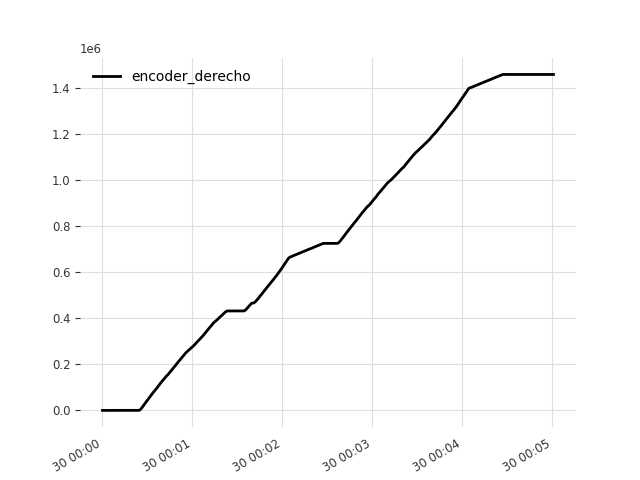
\includegraphics[width=\textwidth]{enc_derecho}
        \caption{Sin procesar}
        \label{fig:datos_enc_derecho_sp}
    \end{subfigure}
    \hfill
    \begin{subfigure}[b]{0.45\textwidth}
        \centering
        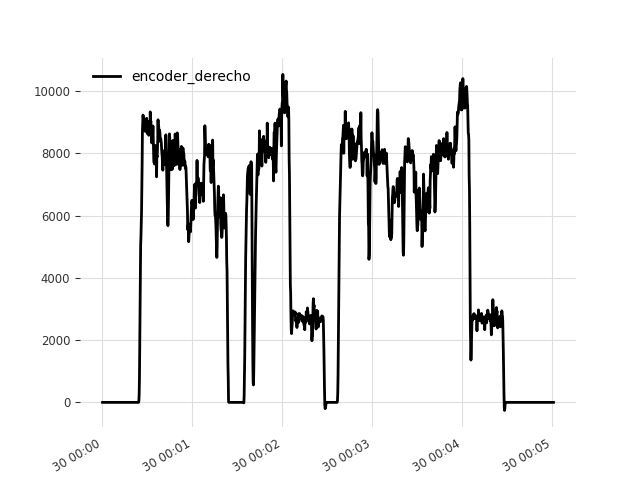
\includegraphics[width=\textwidth]{enc_derecho_dif}
        \caption{Después de diferenciación}
        \label{fig:datos_enc_derecho_dif}
    \end{subfigure}
    \caption{Datos del encoder derecho}
    \label{fig:datos_enc_derecho}
\end{figure}

El objetivo es realizar una predicción de los valores encoder derecho y encoder izquierdo para poder 
compararlos con los obtenidos y detectar posibles errores. Para ello, utilizamos valores anteriores de los 
mismos datos, así como los valores de las consignas de velocidad derecha e izquierda, pues su correlación 
es muy alta. Para predecir los valores derechos, y viceversa, se usan también los valores izquierdos, pues aunque su 
correlación no sea tan alta, también están correlacionados.
Ya que estos datos se mandan en intervalos de tiempo irregulares, el primer paso es agruparlos en ventanas de 200 milisegundos. 
Esto es así porque para realizar las predicciones es necesario que los datos de la serie temporal estén distribuidos 
de manera uniforme.

Las pruebas realizadas a los modelos han sido realizadas únicamente con el encoder derecho, pues al ser muy similar 
al encoder izquierdo se van a obtener resultados prácticamente idénticos en los dos casos, por lo que no merece 
la pena realizar las pruebas sobre los dos datos.

\subsection{Comparativa de modelos de predicción}

Al igual que con la comparativa de sistemas gestores de bases de datos, una comparativa exhaustiva de los modelos 
de predicción puede encontrarse en la sección B.6 de los anexos complementarios.

De dicha comparación se sacan las siguientes conclusiones:
\begin{itemize}
    \item El tiempo empleado para la optimización de los modelos no ha sido suficiente, pues los modelos
        supuestamente optimizados dan peores resultados, tanto en las métricas como en el tiempo de entrenamiento.
    \item El mejor modelo para predicciones a largo plazo es el Transformer por defecto, aunque N-HiTS da buenos
        resultados también con un tiempo de entrenamiento menor.
    \item Para predicciones a corto plazo, ARIMA resulta el mejor modelo.
\end{itemize}

Ya que nuestra intención es realizar predicciones a relativamente largo plazo, el modelo escogido ha sido el modelo 
Transformer. Podría haberse escogido también el modelo N-HiTS, pero como el modelo solo se entrena una vez el tiempo 
de entrenamiento tendrá una menor importancia comparada con el resto de métricas.

\subsection{Desarrollo del servicio}

Como se puede ver en la siguiente imagen (Figura \ref{fig:diagrama_forecast}), este servicio carga un modelo desde 
un archivo o bien lo entrena desde cero. Para poder entrenar dicho modelo, se necesita que la base de datos ya tenga 
datos cargados, por lo que la rutina de entrenamiento espera algunos minutos antes de empezar a entrenar para que 
haya los datos necesarios para poder realizar dicha tarea. La cantidad de tiempo a esperar antes de entrenar se especifica 
en un archivo de configuración.

En el caso de cargar el modelo desde un archivo, también es necesario esperar un tiempo a que la base de datos se cargue 
de información, pues es necesario escalar los datos antes de hacer la predicción. Dicha escala se ajusta según los datos 
introducidos, por lo que cuanto más tiempo esperamos en este paso, más parecida será a la especificada a la hora
de entrenar el modelo.

Los datos generados en la predicción son insertados a un ``bucket'' de la base de datos diferente al que están los datos.
Este ``bucket'' tiene un periodo de retención bajo. Esto significa que los datos insertados se eliminan después 
de cierto tiempo, pues no nos interesa guardar predicciones antiguas.

Existen dos versiones de este servicio: una utiliza una GPU de Nvidia para entrenar y la otra utiliza la CPU. Entrenar con
GPU es mucho más rápido que con CPU, por lo que siempre que se disponga de una es muy recomendable utilizar esta versión.
En caso de no disponer de una GPU, o de disponer de una que no soporte la versión 11.8 de CUDA, siempre puede utilizarse el 
servicio complementario.

\imagen{diagrama_forecast}{Diagrama del servicio de predicción.}{0.8}

\section{Puesta en marcha}

Cada servicio queda definido en un archivo ``Dockerfile'', que definirá el contenido y acciones de cada uno de los 
contenedores.

Todos estos servicios se inician utilizando la herramienta docker compose. Con esta herramienta podremos crear
una red virtual a la que se conectan los diferentes servicios para poder comunicarse entre sí, especificar los
puertos que usa cada contenedor, variables de entorno, volúmenes, etc. Con esta herramienta podemos también ver los registros de cada contenedor, lo que nos permitirá ver posibles errores 
y trazas de información.

\imagen{preds}{Plantilla con los gráficos con las predicciones}{1}

En la Figura \ref{fig:preds} podemos observar las predicciones realizadas en naranja y los datos 
recibidos por el AGV en azul. Una explicación en detalle de como acceder y utilizar esta interfaz se da 
en la sección E.4 de los anexos.
\capitulo{6}{Trabajos relacionados}

Este apartado sería parecido a un estado del arte de una tesis o tesina. En un trabajo final grado no parece obligada su presencia, aunque se puede dejar a juicio del tutor el incluir un pequeño resumen comentado de los trabajos y proyectos ya realizados en el campo del proyecto en curso. 

\capitulo{7}{Conclusiones y Líneas de trabajo futuras}

Todo proyecto debe incluir las conclusiones que se derivan de su desarrollo. Éstas pueden ser de diferente índole, dependiendo de la tipología del proyecto, pero normalmente van a estar presentes un conjunto de conclusiones relacionadas con los resultados del proyecto y un conjunto de conclusiones técnicas. 
Además, resulta muy útil realizar un informe crítico indicando cómo se puede mejorar el proyecto, o cómo se puede continuar trabajando en la línea del proyecto realizado. 



% \bibliographystyle{ieeetr}
% \bibliography{bibliografia}

\printbibliography

\end{document}
